\documentclass{article}
\usepackage{amsfonts, amsmath, amssymb, amsthm} % Math notations imported
\usepackage{enumitem}
\usepackage{graphicx}
\usepackage{setspace}
\usepackage{indentfirst}
\usepackage[margin=1in]{geometry}
\graphicspath{{./images/}} % Path to images

% \begin{figure}[htb!]
%      \centering
%      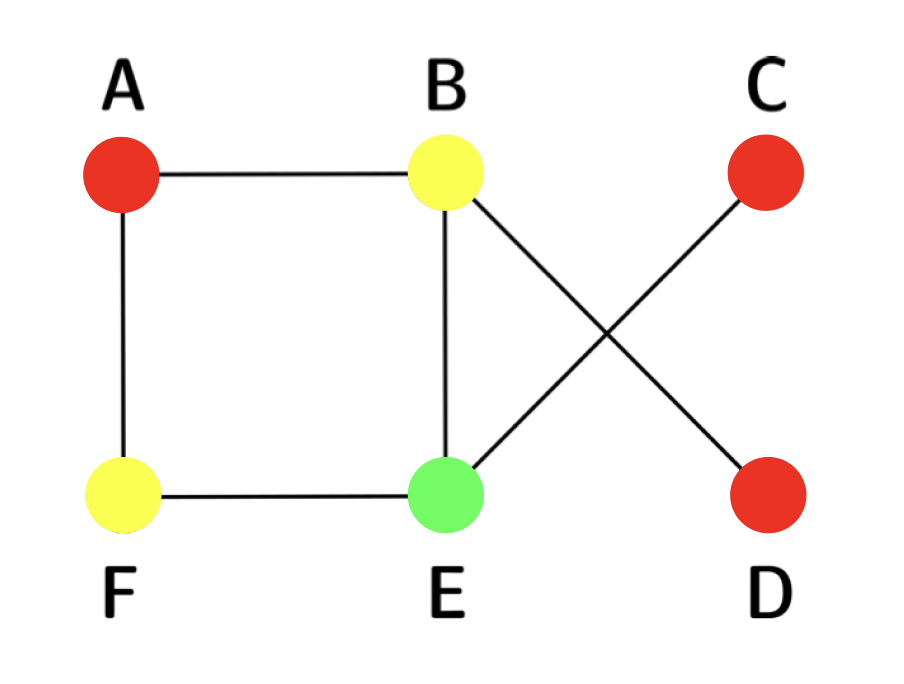
\includegraphics[scale=0.5]{coloring.png}
%      \caption{Coloring of the graph.}
% \end{figure}

% \begin{figure}[htb]
%     \qquad
%     \begin{minipage}{.4\textwidth}
%         \centering
%         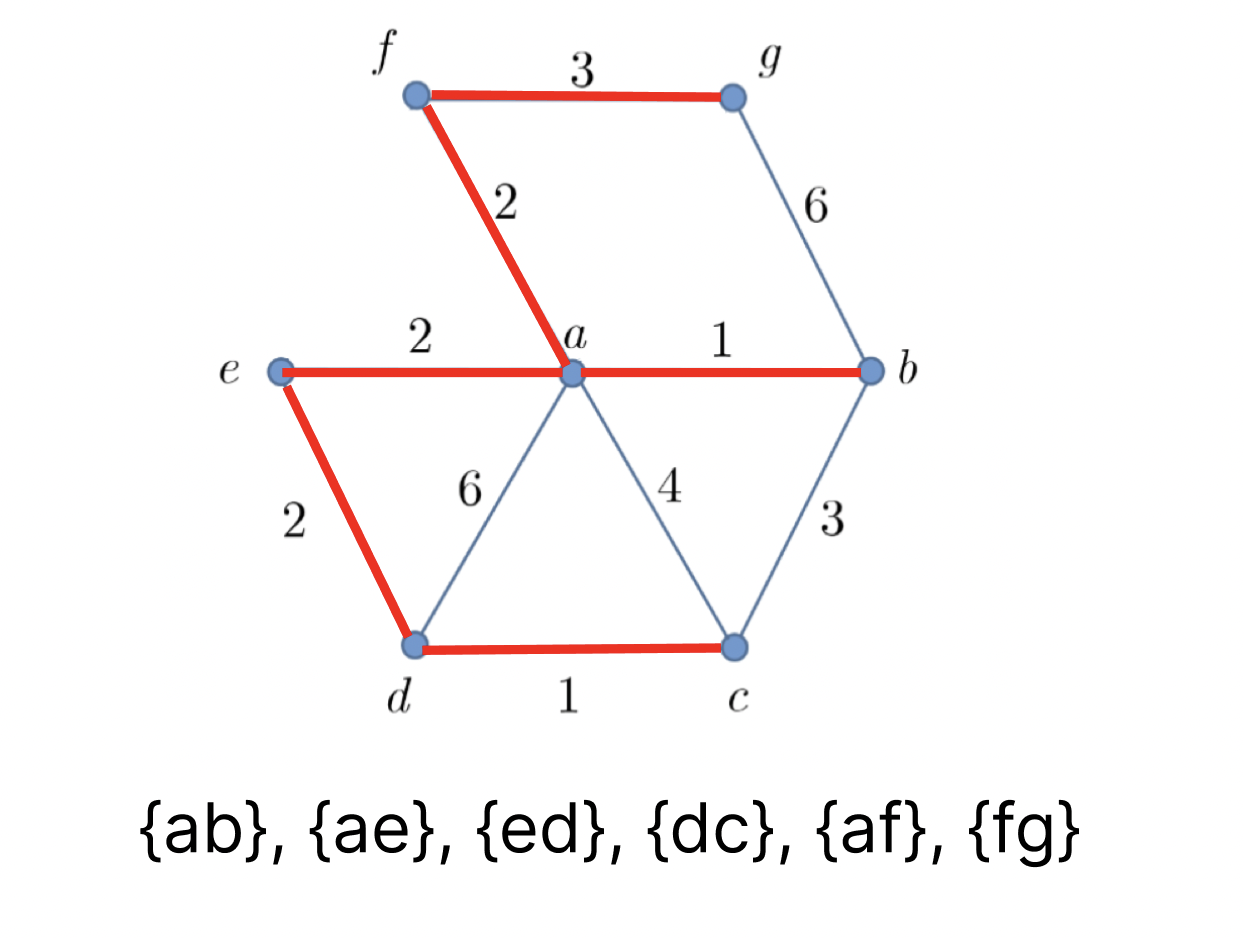
\includegraphics[scale=0.35]{prims.png}
%         \caption{}
%     \end{minipage}    
%     \qquad
%     \begin{minipage}{.4\textwidth}
%         \centering
%         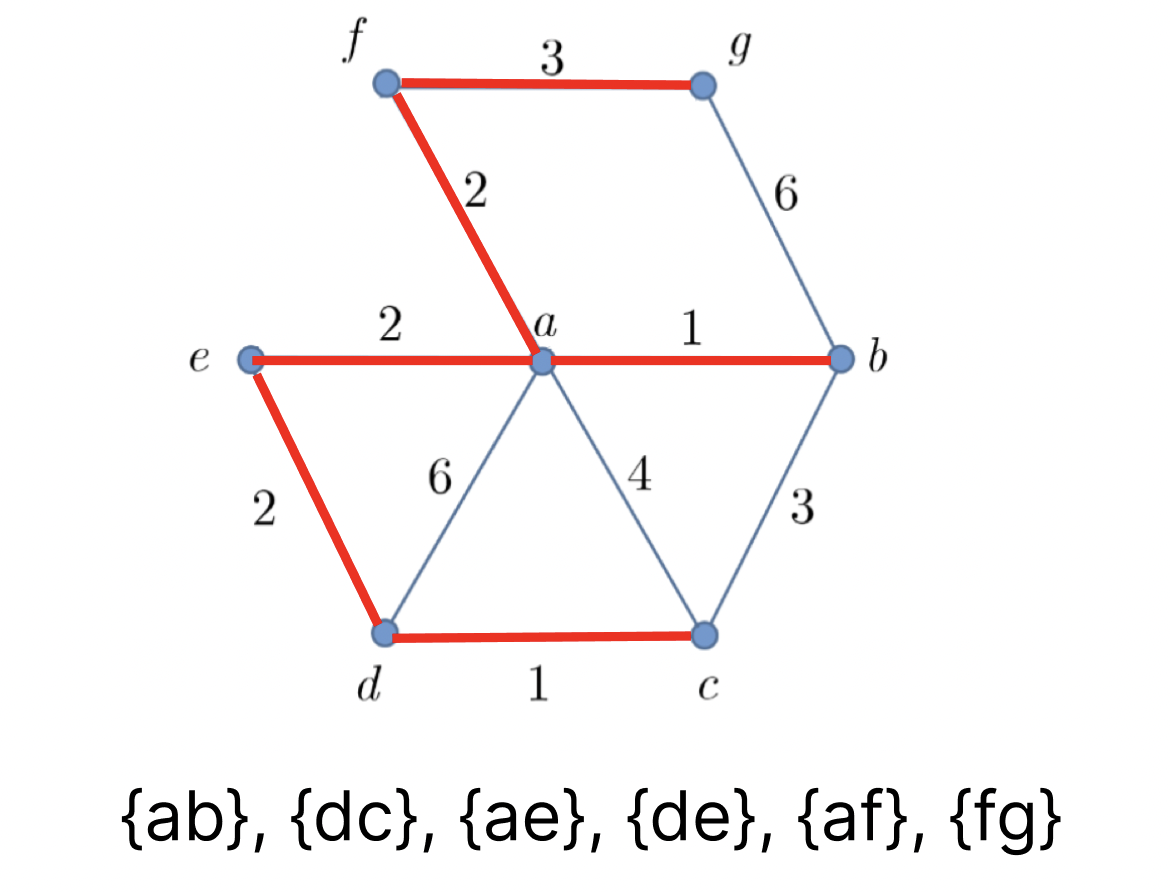
\includegraphics[scale=0.35]{kruskal.png}
%         \caption{}
%     \end{minipage}        
% \end{figure} 

\newtheorem{thm}{Theorem}
\newtheorem{proposition}[thm]{Proposition}
\newtheorem{cor}[thm]{Corollary}

% title information
\title{Math 110 HW3}
\author{Neo Lee}
\date{09/16/2023}

\setstretch{1.15}
% main content
\begin{document} 

% placing title information; comment out if using fancyhdr
\maketitle 

\subsection*{Problem 1}
Let $U:=\{p\in\mathcal{P}_2(\mathbb{R}):\int_{-1}^{1}(xp''(x)+p'(x))dx=0\}.$
\begin{description}
    \item{(a)} Find a basis for $U$. 
    \item{(b)} Extend your basis in part (a) to a basis of ${\mathcal P}_3(\mathbb{R})$.
    \item{(c)} Find a subspace $W$ of ${\mathcal P}_3(\mathbb{R})$ such that ${\mathcal P}_3(\mathbb{R}) = U \oplus W$.
\end{description}

\newpage
\subsection*{Problem 2}
Suppose $v_1, \ldots, v_m$ are linearly independent in $V$ and $w\in V$.  
Prove that $$ \dim span (v_1 - w, v_2 - w, \dots, v_m - w) \ge m-1.$$

\newpage
\subsection*{Problem 3}
Does the `inclusion-exclusion formula' hold for three subspaces, i.e., is it always true that
\begin{eqnarray*} \dim (U_1+U_2+U_3) &= & \dim (U_1)+\dim (U_2)+ \dim (U_3) \\
&&  - \dim (U_1 \cap U_2)- \dim (U_1 \cap U_3)- \dim (U_2 \cap U_3)\\ && + \dim (U_1\cap U_2 \cap U_3)?
\end{eqnarray*} Prove this formula or provide a counterexample.

\newpage
\subsection*{Problem 4}
What is the dimension and the `canonical' basis of:
\begin{description}
\item{(a)}  $\mathbb{C}$ as a vector space over $\mathbb{C}$?  
\item{(b)} $\mathbb{C}$ as a vector space over $\mathbb{R}$? 
\item{(c)} $\mathbb{C}^5$ as a vector space over $\mathbb{C}$?
\item{(d)} $\mathbb{C}^7$ as a vector space over $\mathbb{R}$?
\end{description}

\newpage
\subsection*{Problem 5}
Suppose $U$ and $W$ are subspaces of $V$ such that $U+W=V$, suppose $u_1$, 
$\ldots$, $u_m$ is a basis of $U$ and $w_1$, $\ldots$, $w_n$ is a basis  of $W$. Disprove that 
$u_1$,\ldots, $u_m$, $w_1$, $\ldots$, $w_n$ is necessarily a basis of $V$. What additional 
condition on the sum $U+W$ makes this implication true? Explain.

\end{document}
